% -----------------------------------------------------------------------------
% This source file is part of OSTIS (Open Semantic Technology for Intelligent Systems)
% For the latest info, see http://www.ostis.net
% 
% Copyright (c) 2012 OSTIS
% 
%
% OSTIS is free software: you can redistribute it and/or modify
% it under the terms of the GNU Lesser General Public License as published by
% the Free Software Foundation, either version 3 of the License, or
% (at your option) any later version.
% 
% OSTIS is distributed in the hope that it will be useful,
% but WITHOUT ANY WARRANTY; without even the implied warranty of
% MERCHANTABILITY or FITNESS FOR A PARTICULAR PURPOSE.  See the
% GNU Lesser General Public License for more details.
% 
% You should have received a copy of the GNU Lesser General Public License
% along with OSTIS.  If not, see <http://www.gnu.org/licenses/>.
% -----------------------------------------------------------------------------

\documentclass[hyperref={pdftex,unicode}]{beamer}

\usepackage{latexsym}
\usepackage[warn]{mathtext}     % русские буквы буквы в формулах (с предупреждением)
\usepackage[T2A]{fontenc}
\usepackage[english,russian]{babel}
\usepackage[utf8]{inputenc}

% Подключаем математические формулы
\usepackage{amsmath}
\usepackage{amsfonts}
\usepackage{amssymb}

\usepackage{cmap}               % Поиск по русским буквам в pdf

\usepackage[unicode=true]{hyperref}

\usepackage{rotating}

\usetheme{Warsaw}

\newcommand{\objeqv}{
  \begin{center}
    \begin{sideways}
      \[ \Longleftrightarrow \]
    \end{sideways}
  \end{center}
}

\newcommand{\idtf}[1]{\textit{#1}}

\begin{document}

\title{SC-код в примерах}  
\author{Лазуркин Д.А.}
\date{Минск, 2012} 

\begin{frame}
  \maketitle{}
\end{frame}

% -----------------------------------------------------------------------------
% This source file is part of OSTIS (Open Semantic Technology for Intelligent Systems)
% For the latest info, see http://www.ostis.net
% 
% Copyright (c) 2012 OSTIS
% 
%
% OSTIS is free software: you can redistribute it and/or modify
% it under the terms of the GNU Lesser General Public License as published by
% the Free Software Foundation, either version 3 of the License, or
% (at your option) any later version.
% 
% OSTIS is distributed in the hope that it will be useful,
% but WITHOUT ANY WARRANTY; without even the implied warranty of
% MERCHANTABILITY or FITNESS FOR A PARTICULAR PURPOSE.  See the
% GNU Lesser General Public License for more details.
% 
% You should have received a copy of the GNU Lesser General Public License
% along with OSTIS.  If not, see <http://www.gnu.org/licenses/>.
% -----------------------------------------------------------------------------

\section{Что такое sc-код?}

\begin{frame}{Что такое семантическая сеть?}
  \textbf{Семантическая сеть} — информационная модель предметной
  области, имеющая вид графа, вершины которого соответствуют объектам
  предметной области, а дуги (рёбра) задают отношения между ними.
  \begin{figure}
    \centering
    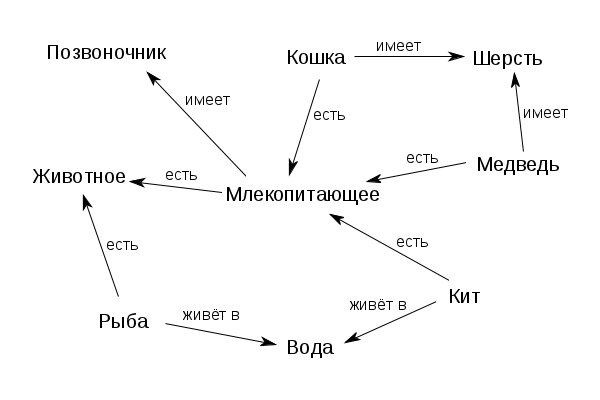
\includegraphics[scale=0.5]{Semantic_net_example}
  \end{figure}
\end{frame}


\begin{frame}{Важные для нас особенности семантических сетей}
  Особенности семантических сетей:
  \begin{itemize}
  \item ориентированы на представление в рафинированом виде `смысла`
    информации
  \item знак каждого объекта описываемой предметной области входит в
    семантическую сеть \textbf{однократно}
  \item каждый объект описываемой предметной области имеет
    неограниченное число связей с другими объектами этой области
  \end{itemize}
\end{frame}


\begin{frame}{Что такое sc-код?}
  \textbf{SC-код} (Semantic Code, абстрактный семантический
  компьютерный код) — универсальный язык бинарных семантических сетей.
  
  Для подачи человеку существует текстовая форма SCs (SC string) и
  графическая форма SCg (SC graphical). В этой презентации я буду
  использовать SCg:
  \begin{figure}
    \centering
    \includegraphics[scale=0.45]{SC_code_example}
  \end{figure}
\end{frame}

\begin{frame}{Текст на SC-коде}
  Семантическая сеть в SC-коде называется \textbf{sc-текстом}
  (\textbf{sc-конструкцией}).  Ниже приведен sc-текст
  (sc-конструкция). Любой элемент в sc-тексте называется
  \textbf{sc-элементом}.
  \begin{figure}
    \centering
    \includegraphics[scale=0.6]{SC_code_example}
  \end{figure}
\end{frame}

\begin{frame}{Узлы sc-конструкции}
  Узел в sc-конструкции называется \textbf{sc-узлом}, который бывает
  различных видов.
  \begin{figure}
    \centering
    \includegraphics[scale=0.6]{SC_code_example_nodes}
  \end{figure}
\end{frame}

\begin{frame}{Связи в sc-конструкции}
  Связь в sc-конструкции в общем случае называется \textbf{sc-коннектором},
  который бывает неориентированным (\textbf{sc-ребро}) и ориентированным
  (\textbf{sc-дуга}).
  \begin{figure}
    \centering
    \includegraphics[scale=0.6]{SC_code_example_connectors}
  \end{figure}
\end{frame}

\begin{frame}{SC-код и теория множеств}
  SC-код основан на теории множеств, поэтому все sc-узлы обозначают
  либо внешние объекты, либо множества, а sc-коннекторы обозначают
  отношения.
  \begin{figure}
    \centering
    \includegraphics[scale=0.6]{SC_code_example}
  \end{figure}
\end{frame}

%%% Local Variables: 
%%% mode: latex
%%% TeX-master: "sc_core_in_examples"
%%% End: 

% -----------------------------------------------------------------------------
% This source file is part of OSTIS (Open Semantic Technology for Intelligent Systems)
% For the latest info, see http://www.ostis.net
% 
% Copyright (c) 2012 OSTIS
% 
%
% OSTIS is free software: you can redistribute it and/or modify
% it under the terms of the GNU Lesser General Public License as published by
% the Free Software Foundation, either version 3 of the License, or
% (at your option) any later version.
% 
% OSTIS is distributed in the hope that it will be useful,
% but WITHOUT ANY WARRANTY; without even the implied warranty of
% MERCHANTABILITY or FITNESS FOR A PARTICULAR PURPOSE.  See the
% GNU Lesser General Public License for more details.
% 
% You should have received a copy of the GNU Lesser General Public License
% along with OSTIS.  If not, see <http://www.gnu.org/licenses/>.
% -----------------------------------------------------------------------------

\section{Формализация в sc-коде}

\subsection{От теории множеств к sc-коду}

\begin{frame}{Множество}
  \begin{center}
    \[ S = \{ \}; \]

    \objeqv  

    \begin{figure}
      \includegraphics{basic/Set}
    \end{figure}
  \end{center}

  \begin{itemize}
  \item такой sc-элемент называется \textbf{константным sc-узлом}
  \item подпись рядом с sс-элементом называется его идентификатором
  \item при помощи такого sc-элемента может обозначаться внешний
    объект, а не только множество
  \end{itemize}
\end{frame}

\begin{frame}{Принадлежность элемента множеству}
  \begin{center}
    \[ a \in S; \] или \[ S = \{ a \}. \]

    \objeqv  

    \begin{figure}
      \includegraphics{basic/El_in_set}
    \end{figure}
  \end{center}

  \begin{itemize}
  \item такой sc-элемент называется \textbf{позитивной константной sc-дугой}
  \end{itemize}
\end{frame}

\begin{frame}{Непринадлежность элемента множеству}
  \begin{center}
    \[ a \notin S \]

    \objeqv  

    \begin{figure}
      \includegraphics{basic/El_not_in_set}
    \end{figure}
  \end{center}

  \begin{itemize}
  \item такой sc-элемент называется \textbf{негативной константной sc-дугой}
  \end{itemize}
\end{frame}

\begin{frame}{Нечеткая принадлежность элемента множеству}
  \begin{figure}
    \centering
    \includegraphics{basic/El_fuzzy_in_set}
  \end{figure}

  \begin{itemize}
  \item такой sc-элемент называется \textbf{нечеткой константной sc-дугой}
  \item используется, когда неизвестна позитивность/негативность sc-дуги
  \end{itemize}
\end{frame}

\begin{frame}{А теперь посмотрим пример покрупнее...}
  \begin{center}
    \[ S = \{S1, S2, S2, a\}; \]
    \[ S1 = \{a, b\}; \]
    \[ S2 = \{b, c, d\}. \]
  \end{center}

  \objeqv

  \begin{figure}
    \includegraphics[scale=0.6]{basic/Complex_sets_example}
  \end{figure}
\end{frame}

\begin{frame}{Сила семантических сетей...}
  \begin{center}
    Честно сказать, я затрудняюсь с ходу написать здесь что-то
    полезное.
  \end{center}

  \objeqv  

  \begin{figure}
    \centering
    \includegraphics{basic/Very_complex_sets_example}
  \end{figure}

  \begin{itemize}
  \item sc-элементы могут не иметь идентификаторов
  \item sc-дуги также могут быть элементами множеств
  \end{itemize}
\end{frame}

\begin{frame}{Кортеж (ориентированное множество)}
  \begin{center}
    \[ T = <a, b, c> \]
    
    \objeqv

    \begin{figure}
      \includegraphics[scale=0.60]{basic/Tuple}
    \end{figure}
  \end{center}

  \begin{itemize}
  \item sc-элемент в виде кружка с крестом внутри называется
    \textbf{атрибутом} и выражает роль объекта в рамках множества
  \item атрибуты \idtf{1\_}, \idtf{2\_}, \idtf{3\_} и т.д. называются
    порядковыми
  \item идентификатор атрибута должен заканчиваться символом "\_"
  \item кортеж в sc-тексте - это множество, каждый элемент которого
    принадлежит ему с указанием определенной роли
  \end{itemize}
\end{frame}

\begin{frame}{Кортеж с нечисловыми атрибутами}
  \begin{center}
    \begin{eqnarray*}
      T = <\cyrmathit{первый}\_: a, \cyrmathit{второй}\_: b, \\
      \cyrmathit{третий}\_: \cyrmathit{дополнительный}\_: c>
    \end{eqnarray*}
    
    \objeqv

    \begin{figure}
      \includegraphics[scale=0.7]{basic/Tuple_with_custom_attrs}
    \end{figure}
  \end{center}

  \begin{itemize}
  \item ролей (атрибутов) у вхождения элемента во множество может быть
    несколько
  \end{itemize}
\end{frame}

\begin{frame}[shrink=20]{Отношение}
  \begin{center}
    \[ R = \{ <a, b>, <c, d> \} \]
    
    \objeqv

    \begin{figure}
      \includegraphics[scale=0.9]{basic/Relation}
    \end{figure}

    \begin{itemize}
    \item для обозначения отношений используется кружок с наклонным
      крестом внутри
    \item sc-элемент в виде кружка с горизонтальной чертой внутри
      называется связкой и выражает связь между своими компонентами
    \item в sc-коде отношение - это множество связок
    \item идентификатор отношения в sc-коде должен обязательно
      заканчиваться символом "*"
    \end{itemize}
  \end{center}
\end{frame}

\begin{frame}{Бинарная ориентированная пара}
  \begin{center}
    \begin{figure}
      \includegraphics{basic/Bin_ord_tuple}
    \end{figure}

    \objeqv

    \begin{figure}
      \includegraphics{basic/Bin_ord_pair}
    \end{figure}
  \end{center}

  \begin{itemize}
  \item так как бинарные связки используются очень часто, то для них
    введен специальный элемент - бинарная ориентированная пара
  \end{itemize}
\end{frame}

\begin{frame}{Отношение c бинарными ориентированными парами}
  \begin{center}
    \begin{figure}
      \includegraphics[scale=0.8]{basic/Relation}
    \end{figure}
    
    \objeqv

    \begin{figure}
      \includegraphics[scale=0.8]{basic/Relation_with_bin_ord_pairs}
    \end{figure}
  \end{center}
\end{frame}

\begin{frame}{Бинарная неориентированная пара}
  \begin{center}
    \begin{figure}
      \includegraphics{basic/Bin_unord_tuple}
    \end{figure}

    \objeqv

    \begin{figure}
      \includegraphics{basic/Bin_unord_pair}
    \end{figure}
  \end{center}

  \begin{itemize}
  \item связка вполне может быть неориентированной
  \item связка - это не всегда кортеж (ориентированное множество)
  \end{itemize}
\end{frame}

\begin{frame}[shrink=5]{Правила формирования идентификаторов sc-элементов}
  \begin{itemize}
  \item если идентификатор начинается с большой буквы, то данный
    sc-элемент обозначает объект с таким именем (имя собственное):
    \begin{itemize}
    \item SC-код
    \item Множество всех возможных чисел
    \item Множество всех студентов
    \item Земля
    \end{itemize}
  \item если идентификатор начинается с маленькой буквы, то данный
    sc-элемент обозначает множество всех объектов с таким именем (имя
    нарицательное):
    \begin{itemize}
    \item число
    \item sc-элемент
    \item студент
    \item планета
    \end{itemize}
  \item идентификатор отношения общего вида должен заканчиваться на символ "*"
  \item идентификатор атрибута должен заканчиваться на символ "\_"
  \end{itemize}
\end{frame}

\begin{frame}{Доп. элемент SCg: Шина}
  \begin{center}
    \begin{figure}
      \includegraphics{basic/Bus_example}
    \end{figure}
  \end{center}
\end{frame}

\begin{frame}{Доп. элемент SCg: Контур}
  \begin{center}
    \begin{figure}
      \includegraphics[scale=0.55]{basic/Contour_example}
    \end{figure}
  \end{center}
\end{frame}

\subsection{Формализация в sc-коде}

\begin{frame}{Виды понятий в sc-коде}
  Понятие (sc-код) - это множество, все элементы которого называются
  экземплярами (объектами) данного понятия.


  При формализации предметной области в sc-коде выделяют следующие
  виды понятий:
  \begin{itemize}
  \item относительное понятие (всегда отношение):
    \begin{itemize}
    \item отношение общего вида
    \item ролевое отношение
    \end{itemize}
  \item абсолютное понятие (все то, что не относительное понятие)
  \end{itemize}
\end{frame}

\begin{frame}{Абсолютное понятие в sc-коде}
  Экземпляр абсолютного понятия никогда не выражает связь между объектами.
  
  \begin{center}
    \begin{figure}
      \includegraphics{basic/Absolute_concept_Number}
    \end{figure}
  \end{center}

  \begin{itemize}
  \item sc-элемент \idtf{число} - это абсолютное понятие, которое
    выражает множество всех чисел
  \item для обозначения абсолютного понятия используется sc-элемент со
    звездой внутри
  \end{itemize}
\end{frame}

\begin{frame}{Абсолютное понятие в sc-коде (sc-структура)}
  Экземпляр абсолютного понятия может состоять из частей, тогда он
  является sc-структурой.
  
  \begin{center}
    \begin{figure}
      \includegraphics{basic/Absolute_concept_Complex_number}
    \end{figure}
  \end{center}

  \begin{itemize}
  \item sc-элемент с точкой внутри - это sc-структура (для простоты
    понимания проведите аналогию со структурами в языках
    программирования)
  \end{itemize}
\end{frame}

\begin{frame}{Относительное понятие в sc-коде (отношение общего вида)}
  \begin{center}
    \begin{figure}
      \includegraphics{basic/Relational_concept_Greater}
    \end{figure}
  \end{center}
\end{frame}

\begin{frame}{Относительное понятие в sc-коде (ролевое отношение)}
  Ролевое (атрибутивное) отношение - это атрибут.

  \begin{center}
    \begin{figure}
      \includegraphics{basic/Absolute_concept_Complex_number}
    \end{figure}
  \end{center}
\end{frame}

\subsection{SC-язык теории множеств}

\begin{frame}{Что такое sc-язык?}
  Набор абсолютных и относительных понятий предметной области задает
  \textbf{sc-язык} данной предметной области. SC-узлы понятий этого
  sc-языка называются его \textbf{ключевыми узлами}.

  Пример sc-языков:
  \begin{itemize}
  \item sc-язык теории множеств
  \item sc-язык логики (SCL, SC Logic)
  \item sc-язык теории графов
  \item sc-язык числовых систем
  \end{itemize}

  Мы рассмотрим некоторые ключевые узлы sc-языка теории множеств.
\end{frame}

\begin{frame}[shrink=10]{Отношение \idtf{включение*} и \idtf{строгое
      включение*}}
  \begin{center}
    \begin{eqnarray*}
      S_1 = \{ a, b, c, d \}; \\
      S_2 = \{ b, c \}; \\
      S_1 \supset S_2; \\
      S_1 \supseteq S_2.
    \end{eqnarray*}

    \objeqv

    \begin{figure}
      \includegraphics[scale=0.7]{basic/Relation_Inclusion_and_Strict_inclusion}
    \end{figure}
  \end{center}

  \begin{itemize}
  \item sc-элементы с одинаковыми идентификаторами склеиваются
  \end{itemize}
\end{frame}

\begin{frame}[shrink=10]{Отношение \idtf{объединение*}}
  \begin{center}
    \begin{eqnarray*}
      S_1 = \{ S_2, a, b \}; \\
      S_2 = \{ b, c, d \}; \\
      S = S_1 \cup S_2 = \{ a, b, c, d, S_2 \}.
    \end{eqnarray*}

    \objeqv

    \begin{figure}
      \includegraphics[scale=0.7]{basic/Relation_Union}
    \end{figure}
  \end{center}
\end{frame}

\begin{frame}[shrink=10]{Отношение \idtf{пересечение*}}
  \begin{center}
    \begin{eqnarray*}
      S_1 = \{ S_2, a, b \}; \\
      S_2 = \{ b, c, d \}; \\
      S = S_1 \cap S_2 = \{ b \}.
    \end{eqnarray*}

    \objeqv

    \begin{figure}
      \includegraphics[scale=0.7]{basic/Relation_Intersection}
    \end{figure}
  \end{center}
\end{frame}

\begin{frame}[shrink=10]{Отношение \idtf{разбиение*}}
  \begin{center}
    \begin{figure}
      \includegraphics[scale=0.7]{basic/Relation_Partition}
    \end{figure}
  \end{center}
\end{frame}

%%% Local Variables: 
%%% mode: latex
%%% TeX-master: "sc_code_in_examples"
%%% End: 

% -----------------------------------------------------------------------------
% This source file is part of OSTIS (Open Semantic Technology for Intelligent Systems)
% For the latest info, see http://www.ostis.net
% 
% Copyright (c) 2012 OSTIS
% 
%
% OSTIS is free software: you can redistribute it and/or modify
% it under the terms of the GNU Lesser General Public License as published by
% the Free Software Foundation, either version 3 of the License, or
% (at your option) any later version.
% 
% OSTIS is distributed in the hope that it will be useful,
% but WITHOUT ANY WARRANTY; without even the implied warranty of
% MERCHANTABILITY or FITNESS FOR A PARTICULAR PURPOSE.  See the
% GNU Lesser General Public License for more details.
% 
% You should have received a copy of the GNU Lesser General Public License
% along with OSTIS.  If not, see <http://www.gnu.org/licenses/>.
% -----------------------------------------------------------------------------

\section{Теория графов в sc-коде}

\begin{frame}{Поиск одного из минимальных путей в неориентированном графе}
  Теперь мы займемся формализацией c использованием sc-кода данных для
  волнового алгоритма поиска одного из минимальных путей в
  неориентированном графе.

  Вся дальнейшая формализация основыввает на базе знаний по теории
  графов
  \href{http://ostisgraphstheo.sourceforge.net/index.php/Заглавная_страница}{OSTIS Graphs Theory}.
\end{frame}

\subsection{Граф в sc-коде}

\begin{frame}{Представление неориентированного графа}
  Начнем мы с представления в sc-коде неориентированного графа $G$:

  \begin{figure}
    \centering
    \includegraphics[scale=0.7]{graph_theory/Undirected_graph_no_scg}
  \end{figure}
\end{frame}

\begin{frame}{Классический математический способ задания графа}
  Классический математический способ задания графа $G$ будет выглядеть
  следующим образом:
  
  \[ G = <Vertex, Edge>; \]
  \[ Vertex = \{ A, B, C, E, D, F, K \}; \]
  \[ Edge = \{ \{A, B\}, \{A, C\}, \{C, E\}, \{C, D\}, \{B, E\}, \{E, F\} \}. \]
\end{frame}

\begin{frame}{Абсолютное понятия `Неориентированный граф`}
  Для представления неориентированных графов в sc-коде введем
  абсолютное понятия \idtf{неориентированный граф}, т.е. множество
  всех неориентированных графов.
  Тогда граф G в sc-коде будет выглядеть следующим образом...
\end{frame}

\begin{frame}{Классический способ задания неориентированного графа (sc-код)}
  \begin{figure}
    \centering
    \includegraphics[scale=0.6]{graph_theory/Undirected_graph_classic}
  \end{figure}
\end{frame}

\begin{frame}{Основной способ задания неориентированного граф}
  Давайте введем два относительных понятия (ролевых отношения)
  \idtf{вершина\_} и \idtf{ребро\_}, тогда граф $G$ на языке теории множеств можно
  задать следующим образом:

  \begin{eqnarray*}
    G = <\cyrmathit{вершина}\_: A, \cyrmathit{вершина}\_: B, \\
    \cyrmathit{вершина}\_: C, \cyrmathit{вершина}\_: E, \\
    \cyrmathit{вершина}\_: D, \cyrmathit{вершина}\_: F, \\
    \cyrmathit{вершина}\_: K, \cyrmathit{ребро}\_: \{A, B\}, \\
    \cyrmathit{ребро}\_: \{A, C\}, \cyrmathit{ребро}\_: \{C, E\}, \\
    \cyrmathit{ребро}\_: \{C, D\}, \cyrmathit{ребро}\_: \{B, E\}, \\
    \cyrmathit{ребро}\_: \{E, F\}>.
  \end{eqnarray*}
\end{frame}

\begin{frame}{Основная способ задания неориентированного графа (sc-код)}
  \begin{figure}
    \centering
    \includegraphics[scale=0.6]{graph_theory/Undirected_graph_main}
  \end{figure}
\end{frame}

\begin{frame}{Представление ориентированного графа}
  Теперь попробуем представить в sc-коде ориентированного графа $G_d$:

  \begin{figure}
    \centering
    \includegraphics[scale=0.7]{graph_theory/Directed_graph_no_scg}
  \end{figure}
\end{frame}

\begin{frame}{Представление неориентированного графа (доп. понятия)}
  Для представления графа $G_d$ введем абсолютное понятие
  \idtf{ориентированный граф} и относительное понятия (ролевое отношение)
  \idtf{дуга\_}.
\end{frame}

\begin{frame}{Представление ориентированного графа (sc-код)}
  \begin{figure}
    \centering
    \includegraphics[scale=0.6]{graph_theory/Directed_graph}
  \end{figure}
\end{frame}

\begin{frame}{Сокращенная форма представления графа (sc-код)}
  Для удобства восприятия графа человеком (\emph{но не машиной})
  будем в дальнейшем максимальным образом использовать сокращенную
  форму задания графа:
  
  \begin{figure}
    \centering
    \includegraphics[scale=0.6]{graph_theory/Undirected_graph_short_form}
  \end{figure}
\end{frame}

\subsection{Минимальный путь в sc-коде}

\begin{frame}{Определение маршрута}
  Из книги Ф. Харрари `Теория графов` (глава `Маршруты и связность`, с. 26):
  \begin{quote}
    \textbf{Маршрутом} в графе $G$ называется чередующаяся последовательность
    вершин и ребер $v_0$, $x_1$, $v_1$, …, $v_{n-1}$, $x_n$, $v_n$; эта последовательность
    начинается и кончается вершиной, и каждое ребро последовательности
    инцидентно двум вершинам, одна из которых непосредственно
    предшествует ему, а другая непосредственно следует за
    ним. Указанный маршрут соединяет вершины $v_0$ и $v_n$, и его можно
    обозначить $v_0$, $v_1$, …, $v_n$ (наличие ребер подразумевается).
  \end{quote}
\end{frame}

\begin{frame}{Определение пути}
  Из книги Ф. Харрари `Теория графов` (глава `Маршруты и связность`, с. 26):
  \begin{quote}
    Маршрут называется \textbf{цепью}, если все его ребра различны, и
    \textbf{простой цепью} (\textbf{путем}), если все вершины (а,
    следовательно, и ребра) различны.
  \end{quote}
\end{frame}

\begin{frame}{Пример пути в графе}
  В графе $G$ выделен синем цветом пути $R$, который задается
  последовательностью $A$, $e_2$, $B$, $e_5$, $E$, $e_6$, $F$:
  \begin{figure}
    \centering
    \includegraphics[scale=0.7]{graph_theory/Path_example_no_scg}
  \end{figure}
\end{frame}

\begin{frame}{Путь - это маршрут}
  Так как путь - это маршрут, то, определив более общее понятие, мы
  разберемся с более частным.

  Маршрут - это относительное понятие, которое связывает граф с
  некоторой последовательностью (структурой маршрута).

  Введем бинарное ориентированное отношение \idtf{маршрут*}:
  \begin{figure}
    \centering
    \includegraphics{graph_theory/Example_of_relations_Route_tuple}
  \end{figure}
\end{frame}

\begin{frame}{Различные способы представления маршрута}
  Мы будем рассматривать следующие способы представления структуры
  маршрута:
  \begin{itemize}
  \item подграф
  \item последовательность
  \item соответствие
  \end{itemize}
\end{frame}

\subsubsection{Маршрут, как подграф}

\begin{frame}{Отношение \idtf{подграф*}}
  Пример бинарного ориентированного отношения \idtf{подграф*},
  которое связывает граф $G_1$ с его подграфом $G_2$:
  \begin{figure}
    \centering
    \includegraphics{graph_theory/Relation_Subgraph_example}
  \end{figure}
\end{frame}

\begin{frame}{Маршрут $R$, как подграф}
  \begin{figure}
    \centering
    \includegraphics[scale=0.60]{graph_theory/Route_as_subgraph}
  \end{figure}
\end{frame}

\begin{frame}{Проблема представления маршрута в виде подграфа}
  \begin{figure}
    \centering
    \includegraphics[scale=0.60]{graph_theory/Route_as_subgraph_problem}
  \end{figure}
\end{frame}

\subsubsection{Маршрут, как последовательность}

\begin{frame}{Маршрут $R$, как поcледовательность}
  \begin{figure}
    \centering
    \includegraphics[scale=0.60]{graph_theory/Route_as_sequence}
  \end{figure}
\end{frame}

\subsubsection{Маршрут, как соответствие}

\begin{frame}{От вершин и ребер к посещениям вершин и ребер}
  Снова заглянем в Ф. Харрари `Теория графов` (глава `Маршруты и связность`, с. 26):
  \begin{quote}
    \textbf{Маршрутом} в графе $G$ называется чередующаяся последовательность
    вершин и ребер $v_0$, $x_1$, $v_1$, \dots, $v_{n-1}$, $x_n$, $v_n$; \dots
  \end{quote}

  Давайте сделаем явным в этом определении то, что якобы считается
  само собой разумеющимся:
  \begin{quote}
    \textbf{Маршрутом} в графе $G$ называется чередующаяся последовательность \textbf{посещений}
    вершин и ребер $v_0$, $x_1$, $v_1$, \dots, $v_{n-1}$, $x_n$, $v_n$; \dots
  \end{quote}
\end{frame}

\begin{frame}{Структура маршрута $R$}
  \begin{figure}
    \centering
    \includegraphics[scale=0.55]{graph_theory/Route_as_correspondence_incomplete}
  \end{figure}
\end{frame}

\begin{frame}{Пример отношения \idtf{соответствие*}}
  \begin{figure}
    \centering
    \includegraphics[scale=0.65]{graph_theory/Relation_Correspondece_example}
  \end{figure}
\end{frame}

\begin{frame}{Маршрут $R$, как соответствие}
  \begin{figure}
    \centering
    \includegraphics[scale=0.50]{graph_theory/Route_as_correspondence_final}
  \end{figure}
\end{frame}

\subsubsection{Минимальный путь в графе}

\begin{frame}{Отношения \idtf{цепь*} и \idtf{путь*} (\idtf{простая цепь*})}
  \begin{figure}
    \centering
    \includegraphics{graph_theory/Relations_Trail_Path}
  \end{figure}
\end{frame}

\begin{frame}{Один из минимальных путей в графе $G$}
  \begin{figure}
    \centering
    \includegraphics[scale=0.54]{graph_theory/Path_final}
  \end{figure}
\end{frame}

\subsection{Обобщение различных видов графов}

\begin{frame}{Пример абсолютного понятия \idtf{графовая структура}}
  \begin{figure}
    \centering
    \includegraphics[scale=0.7]{graph_theory/Graph_structure_example}
  \end{figure}
\end{frame}

\begin{frame}{Иерархия типов \idtf{графовых структур}}
  \begin{figure}
    \centering
    \includegraphics[scale=0.55]{graph_theory/Hierarchy_of_graphs_types}
  \end{figure}
\end{frame}

\begin{frame}{Иерархия ролей элементов \idtf{графовых структур}}
  \begin{figure}
    \centering
    \includegraphics[scale=0.43]{graph_theory/Hierarchy_of_elements_roles_in_graph_structure}
  \end{figure}
\end{frame}

%%% Local Variables: 
%%% mode: latex
%%% TeX-master: "sc_code_in_examples"
%%% End: 


\end{document}
